\chapter{Vectores Contextualizados}

\begin{planningbox}{Bloque C06}
En este capitulo los vectores aparecen como herramientas de representacion de desplazamientos,
fuerzas, orientaciones y construcciones geometricas. El foco es interpretar las coordenadas,
no tratarlas como una lista de numeros sin significado.
\end{planningbox}

\section{[C06.S01] Bases y dependencia en \texorpdfstring{\(\R^2\)}{R2}}

\begin{exercise}{[CTX-C06.S01-01] Desplazamiento en una base oblicua}
Un robot de almacen no se mueve en los ejes cartesianos habituales, sino segun dos carriles
oblicuos cuyas direcciones base son
\[
\vec u=(2,1),\qquad \vec v=(1,2).
\]

En una maniobra debe alcanzar el desplazamiento total
\[
\vec d=(11,10).
\]
Determina:
\begin{enumerate}
  \item si \(\vec u\) y \(\vec v\) forman una base de \(\R^2\);
  \item cuantos tramos de cada carril debe recorrer el robot para reproducir \(\vec d\).
\end{enumerate}
\end{exercise}

\begin{shortanswer}{[CTX-C06.S01-01]}
Si, porque los vectores son linealmente independientes. El desplazamiento se escribe como
\[
\vec d=4\vec u+3\vec v.
\]
\end{shortanswer}

\begin{fullsolution}{[CTX-C06.S01-01]}
Los vectores forman una base si son linealmente independientes. Calculamos el determinante
\[
\det\begin{pmatrix}2&1\\1&2\end{pmatrix}=4-1=3\neq 0.
\]
Por tanto, \(\vec u\) y \(\vec v\) forman una base de \(\R^2\).

Buscamos escalares \(a,b\) tales que
\[
a(2,1)+b(1,2)=(11,10).
\]
Esto da el sistema
\[
\begin{cases}
2a+b=11,\\
a+2b=10.
\end{cases}
\]
De la segunda ecuacion,
\[
a=10-2b.
\]
Sustituyendo en la primera:
\[
2(10-2b)+b=11
\Longrightarrow
20-3b=11
\Longrightarrow
b=3.
\]
Entonces
\[
a=10-6=4.
\]
Por tanto,
\[
\vec d=4\vec u+3\vec v.
\]
\end{fullsolution}

\section{[C06.S02] Operaciones con vectores}

\begin{exercise}{[CTX-C06.S02-01] Ruta compuesta de un dron}
Durante una inspeccion, un dron realiza tres desplazamientos sucesivos, en metros:
\[
\vec u=(6,-1),\qquad \vec v=(2,5),\qquad \vec w=(-4,3).
\]

Calcula:
\begin{enumerate}
  \item el desplazamiento total;
  \item el vector de correccion necesario para volver al punto de salida en linea recta;
  \item la longitud de esa correccion.
\end{enumerate}
\end{exercise}

\begin{databox}{Esquema del recorrido}
\begin{center}
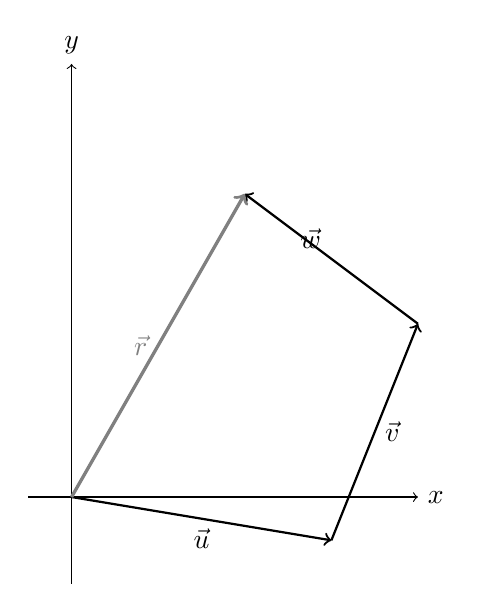
\begin{tikzpicture}[scale=0.55]
  \draw[->] (-1,0) -- (8,0) node[right] {\(x\)};
  \draw[->] (0,-2) -- (0,10) node[above] {\(y\)};
  \draw[->,thick] (0,0) -- (6,-1) node[midway,below] {\(\vec u\)};
  \draw[->,thick] (6,-1) -- (8,4) node[midway,right] {\(\vec v\)};
  \draw[->,thick] (8,4) -- (4,7) node[midway,above left] {\(\vec w\)};
  \draw[->,very thick,gray] (0,0) -- (4,7) node[midway,left] {\(\vec r\)};
\end{tikzpicture}
\end{center}
\end{databox}

\begin{shortanswer}{[CTX-C06.S02-01]}
El desplazamiento total es
\[
\vec r=(4,7).
\]
La correccion de vuelta es
\[
(-4,-7),
\]
y su longitud es
\[
\sqrt{65}\approx \SI{8.06}{m}.
\]
\end{shortanswer}

\begin{fullsolution}{[CTX-C06.S02-01]}
Sumamos coordenadas:
\[
\vec r=\vec u+\vec v+\vec w=(6,-1)+(2,5)+(-4,3)=(4,7).
\]
Para volver al origen en linea recta hace falta aplicar el vector opuesto:
\[
\vec c=-\vec r=(-4,-7).
\]
La longitud de la correccion es
\[
\|\vec c\|=\sqrt{(-4)^2+(-7)^2}=\sqrt{16+49}=\sqrt{65}\approx \SI{8.06}{m}.
\]
\end{fullsolution}

\section{[C06.S03] Modulo, argumento y vectores unitarios}

\begin{exercise}{[CTX-C06.S03-01] Vector de viento dominante}
Una estacion meteorologica registra un vector de viento
\[
\vec v=(-6,6\sqrt{3}).
\]

Determina:
\begin{enumerate}
  \item el modulo del viento;
  \item su argumento en grados y en radianes;
  \item el vector unitario asociado.
\end{enumerate}
\end{exercise}

\begin{shortanswer}{[CTX-C06.S03-01]}
\[
\|\vec v\|=12,
\qquad
\arg(\vec v)=120^\circ=\frac{2\pi}{3}.
\]
El vector unitario es
\[
\left(-\frac12,\frac{\sqrt3}{2}\right).
\]
\end{shortanswer}

\begin{fullsolution}{[CTX-C06.S03-01]}
El modulo es
\[
\|\vec v\|=\sqrt{(-6)^2+(6\sqrt3)^2}=\sqrt{36+108}=\sqrt{144}=12.
\]
El vector esta en el segundo cuadrante. Su angulo de referencia \(\beta\) cumple
\[
\tg\beta=\left|\frac{6\sqrt3}{-6}\right|=\sqrt3,
\]
asi que
\[
\beta=60^\circ.
\]
En el segundo cuadrante,
\[
\arg(\vec v)=180^\circ-60^\circ=120^\circ=\frac{2\pi}{3}.
\]
El vector unitario asociado es
\[
\frac{\vec v}{\|\vec v\|}=
\left(\frac{-6}{12},\frac{6\sqrt3}{12}\right)=
\left(-\frac12,\frac{\sqrt3}{2}\right).
\]
\end{fullsolution}

\section{[C06.S04] Producto escalar y angulo entre vectores}

\begin{exercise}{[CTX-C06.S04-01] Dos fuerzas de arrastre}
Dos remolcadores ejercen fuerzas proporcionales a los vectores
\[
\vec u=(6,2),
\qquad
\vec v=(3,7).
\]

Calcula:
\begin{enumerate}
  \item el producto escalar;
  \item el angulo entre ambas fuerzas;
  \item si la accion conjunta es mas bien cooperativa o antagonica.
\end{enumerate}
\end{exercise}

\begin{shortanswer}{[CTX-C06.S04-01]}
\[
\vec u\cdot \vec v=32,
\qquad
\cos\theta=\frac{8}{\sqrt{145}}.
\]
El angulo es aproximadamente \(48.3^\circ\), asi que la accion es cooperativa.
\end{shortanswer}

\begin{fullsolution}{[CTX-C06.S04-01]}
El producto escalar es
\[
\vec u\cdot \vec v=6\cdot 3+2\cdot 7=18+14=32.
\]
Los modulos valen
\[
\|\vec u\|=\sqrt{6^2+2^2}=\sqrt{40}=2\sqrt{10},
\qquad
\|\vec v\|=\sqrt{3^2+7^2}=\sqrt{58}.
\]
Por la formula del producto escalar,
\[
\cos\theta=
\frac{\vec u\cdot \vec v}{\|\vec u\|\,\|\vec v\|}=
\frac{32}{2\sqrt{10}\sqrt{58}}=
\frac{32}{4\sqrt{145}}=
\frac{8}{\sqrt{145}}.
\]
Por tanto,
\[
\theta\approx \arccos\left(\frac{8}{\sqrt{145}}\right)\approx 48.3^\circ.
\]
Como el angulo es agudo, las fuerzas apuntan en direcciones compatibles y su accion conjunta
es cooperativa, no antagonica.
\end{fullsolution}

\section{[C06.S05] Paralelismo, perpendicularidad y alineacion}

\begin{exercise}{[CTX-C06.S05-01] Sensores alineados y corredor perpendicular}
Tres sensores estan situados en
\[
A(1,2),\qquad B(5,5),\qquad C(9,8).
\]
Desde \(C\) parte un corredor de servicio hasta \(D(12,4)\).

Comprueba:
\begin{enumerate}
  \item si \(A\), \(B\) y \(C\) estan alineados;
  \item si el corredor \(CD\) es perpendicular a la alineacion de los sensores.
\end{enumerate}
\end{exercise}

\begin{shortanswer}{[CTX-C06.S05-01]}
Los tres sensores estan alineados porque
\[
\overrightarrow{AB}=(4,3),\qquad \overrightarrow{BC}=(4,3).
\]
Ademas,
\[
\overrightarrow{CD}=(3,-4),
\]
y se cumple
\[
(4,3)\cdot(3,-4)=0,
\]
asi que el corredor es perpendicular.
\end{shortanswer}

\begin{fullsolution}{[CTX-C06.S05-01]}
Calculamos
\[
\overrightarrow{AB}=(5-1,5-2)=(4,3),
\]
\[
\overrightarrow{BC}=(9-5,8-5)=(4,3).
\]
Como \(\overrightarrow{AB}\) y \(\overrightarrow{BC}\) son iguales, los puntos \(A\), \(B\) y
\(C\) estan alineados.

Ahora
\[
\overrightarrow{CD}=(12-9,4-8)=(3,-4).
\]
El producto escalar con la direccion de la recta de sensores es
\[
(4,3)\cdot(3,-4)=12-12=0.
\]
Por tanto, el corredor \(CD\) es perpendicular a la alineacion de los sensores.
\end{fullsolution}

\section{[C06.S06] Construcciones con vectores y paralelogramos}

\begin{exercise}{[CTX-C06.S06-01] Plataforma paralelogramica}
En una plataforma de carga se conocen tres vertices de un paralelogramo:
\[
A(1,1),\qquad B(7,2),\qquad D(3,6),
\]
donde \(AB\) y \(AD\) son lados consecutivos.

Calcula:
\begin{enumerate}
  \item el cuarto vertice \(C\);
  \item el punto de corte de las diagonales;
  \item el area del paralelogramo.
\end{enumerate}
\end{exercise}

\begin{databox}{Croquis de la plataforma}
\begin{center}
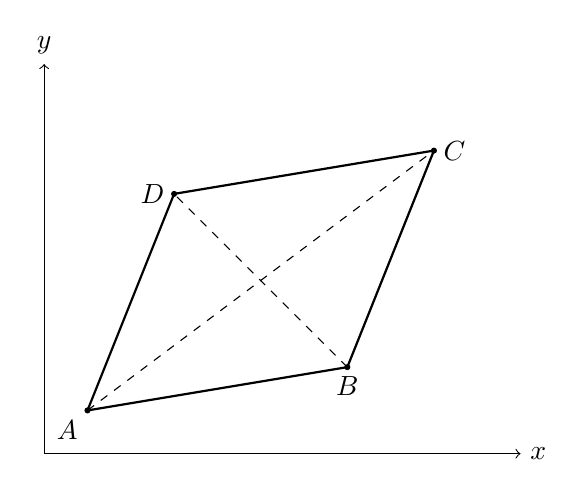
\begin{tikzpicture}[scale=0.55]
  \draw[->] (0,0) -- (11,0) node[right] {\(x\)};
  \draw[->] (0,0) -- (0,9) node[above] {\(y\)};
  \draw[thick] (1,1) -- (7,2) -- (9,7) -- (3,6) -- cycle;
  \draw[dashed] (1,1) -- (9,7);
  \draw[dashed] (7,2) -- (3,6);
  \fill (1,1) circle (2pt) node[below left] {\(A\)};
  \fill (7,2) circle (2pt) node[below] {\(B\)};
  \fill (9,7) circle (2pt) node[right] {\(C\)};
  \fill (3,6) circle (2pt) node[left] {\(D\)};
\end{tikzpicture}
\end{center}
\end{databox}

\begin{shortanswer}{[CTX-C06.S06-01]}
\[
C=B+D-A=(9,7),
\qquad
M=\left(5,4\right).
\]
El area del paralelogramo es \(28\) unidades cuadradas.
\end{shortanswer}

\begin{fullsolution}{[CTX-C06.S06-01]}
Como en un paralelogramo
\[
\overrightarrow{AC}=\overrightarrow{AB}+\overrightarrow{AD},
\]
se puede calcular \(C\) mediante
\[
C=B+D-A.
\]
Entonces
\[
C=(7,2)+(3,6)-(1,1)=(9,7).
\]

Las diagonales se cortan en su punto medio, asi que
\[
M=\frac{A+C}{2}=
\left(\frac{1+9}{2},\frac{1+7}{2}\right)=(5,4).
\]

Para el area usamos el determinante de los lados consecutivos:
\[
\overrightarrow{AB}=(6,1),
\qquad
\overrightarrow{AD}=(2,5).
\]
Luego
\[
Area=\left|\det
\begin{pmatrix}
6 & 1\\
2 & 5
\end{pmatrix}
\right|
=|6\cdot 5-1\cdot 2|=|30-2|=28.
\]
\end{fullsolution}
